\documentclass[english]{article}
\usepackage{graphicx}
\usepackage[left = 20mm, right=20mm, top=25mm,bottom=25mm]{geometry}
\usepackage{babel}
\begin{document}
Comparing plots for two instances of machine learning- weighted vs unweighted.\\
Signal-Spin0p\\
Background-Spin0m
\begin{figure}[!htb]
\minipage{.5\textwidth}
	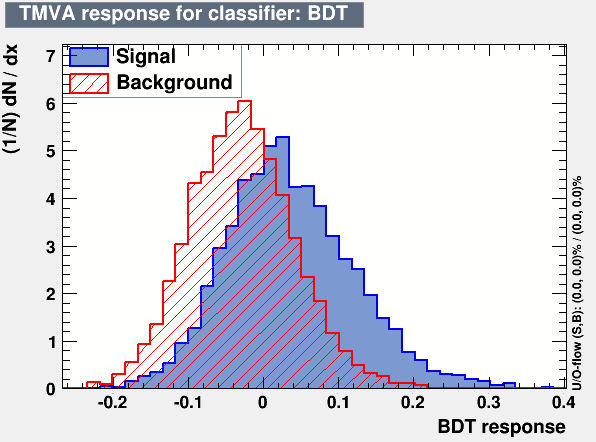
\includegraphics[width=\linewidth]{BDT_t_u}
	\caption{Plot for BDT (test sample) from unweighted TMVA analysis}
\endminipage\hfill
\minipage{.5\textwidth}
	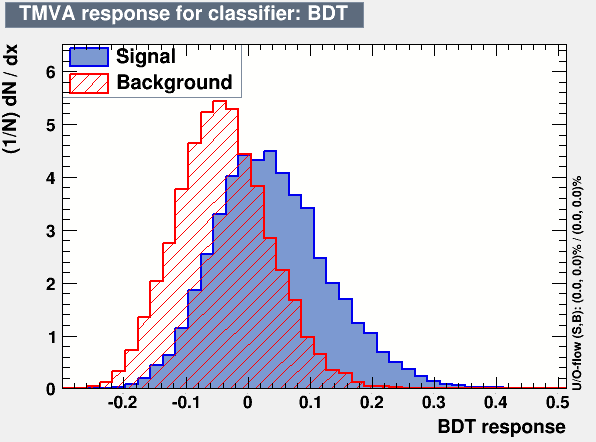
\includegraphics[width=\linewidth]{BDT_t_w}
	\caption{Plot for BDT(test sample) from weighted TMVA analysis}
\endminipage\hfill
\end{figure}


\begin{figure}[!htb]
\minipage{.5\textwidth}
	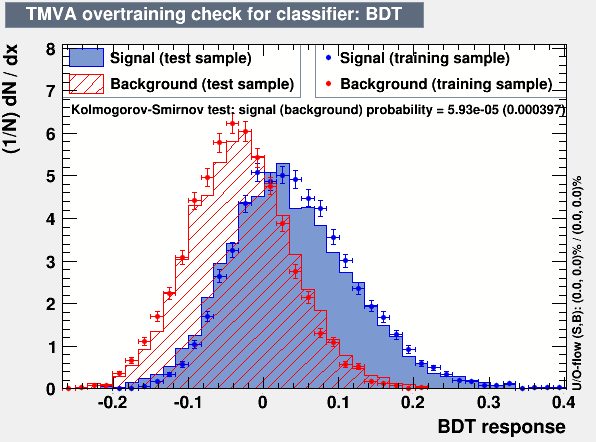
\includegraphics[width=\linewidth]{BDT_tt_u}
	\caption{Plot for BDT(test and training) from unweighted TMVA analysis}
\endminipage\hfill
\minipage{.5\textwidth}
	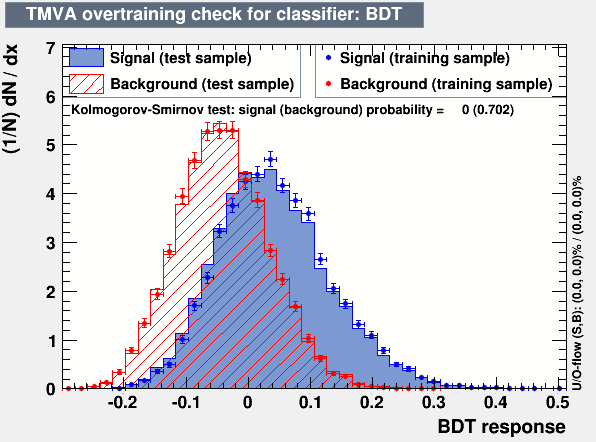
\includegraphics[width=\linewidth]{BDT_tt_w}
	\caption{Plot for BDT(test and training) from weighted TMVA analysis}
\endminipage\hfill
\end{figure}

\newpage
Plots for Background rejection(Spin0m) vs Signal efficiency(Spin0p)\\
\begin{figure}[!htb]
\minipage{.5\textwidth}
        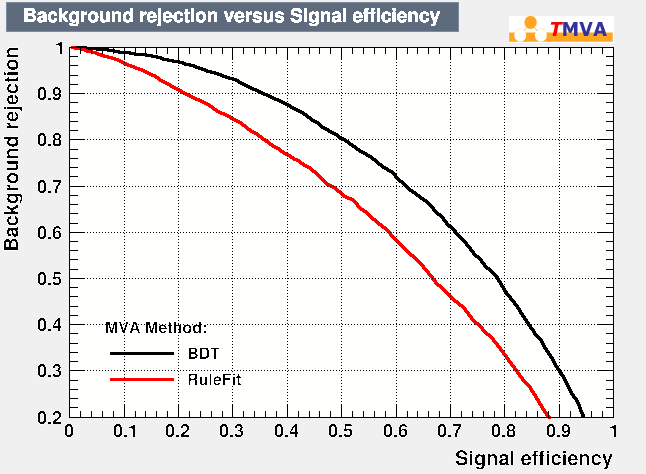
\includegraphics[width=\linewidth]{bksig_roc_u}
        \caption{Background rejection vs signal efficiency curve for unweighted}
\endminipage\hfill
\minipage{.5\textwidth}
        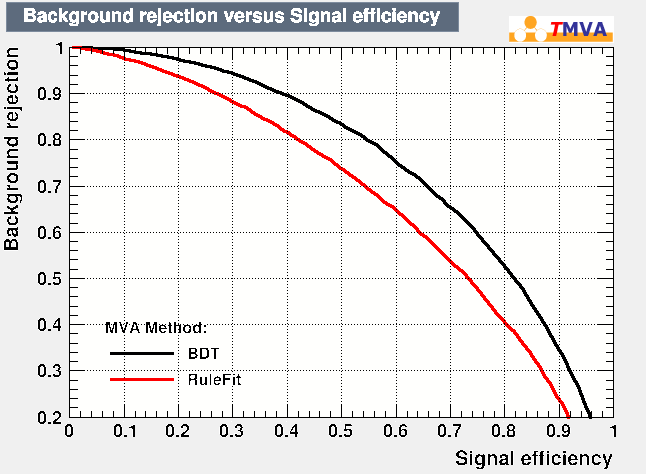
\includegraphics[width=\linewidth]{bksig_roc_w}
        \caption{Background rejection vs signal efficiency curve for weighted}
\endminipage\hfill
\end{figure}

\end{document}
